\section{Rethinking Where Diffusion Models Underfit} \label{sec:extrapolation}
In this section, we challenge the standard \common from \Cref{sec:background} that diffusion models learn globally over the entire data space. Instead, we decompose the diffusion model learning into two regions: they are `supervised' on a restricted region, and forced to `extrapolate' beyond this region during inference. To motivate this, we begin with a paradox arising from Classifier-Free Guidance~\citepn{CFG}{ho2022classifier}, which \common cannot explain.

\begin{minipage}{0.613\textwidth}
\begin{example}[CFG Paradox] \label{example:cfg}
    CFG jointly trains conditional \& unconditional models $\rvs_\rvtheta (\cdot, \cdot, c)$ \& $\rvs_\rvtheta (\cdot, \cdot, \varnothing)$, and samples with the combined CFG score to improve sample quality:
    \begin{equation*}
        \rvs_{\text{CFG}}^\omega := \rvs_\rvtheta (\rvz_t, t, c) + (\omega - 1) \xxpurple{\left[\rvs_\rvtheta (\rvz_t, t, c) - \rvs_\rvtheta (\rvz_t, t, \varnothing) \right]}
        % \vspace{-5pt}
    \end{equation*}
    CFG works because the \emph{difference between conditional and unconditional scores} is recognizable; if these scores are identical, CFG reduces to standard conditional sampling. Indeed, these two learned scores \emph{differ meaningfully during inference} (\Cref{fig:cfg-paradox}, \coloreddashul{xred}{red line}). According to \common, both learned scores should globally approximate their empirical counterparts on conditional and unconditional training data: $\rvs_\rvtheta (\rvz_t, t, c) \approx \rvs_\star^{c}(\rvz_t, t)$ and $\rvs_\rvtheta (\rvz_t, t, \varnothing) \approx \rvs_\star^{\varnothing} (\rvz_t, t)$. Measuring the difference between the empirical scores, however, \xxpurple{$\| \rvs_\star^{c} - \rvs_\star^{\varnothing} \|$} over $\rvz_t \sim \hat{p}_t$, we find it is \emph{vanishingly small during training} for most timesteps (\Cref{fig:cfg-paradox}, \coloreddashul{xblue}{blue line}). This leads to a paradox: why is there such a discrepancy?
\end{example}
\end{minipage}
\hfill
\begin{minipage}{0.367\textwidth}
   \begin{figure}[H]
    \centering
    \vskip -\baselineskip
    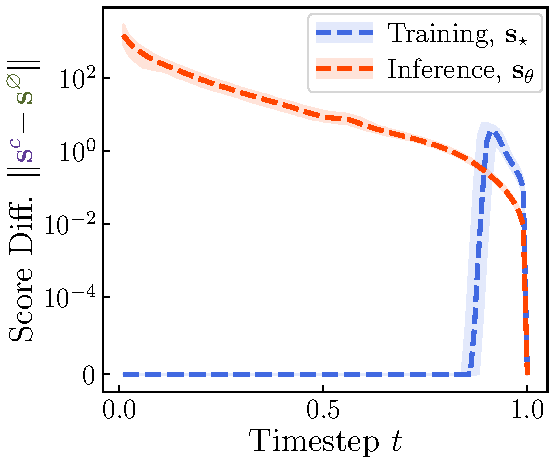
\includegraphics[width=\textwidth,trim={0.1cm 0 0 0}]{figures/extrapolation/cfg_paradox}
    \vskip -0.7\baselineskip
    \caption{\textbf{Difference between \xxpurple{conditional} and \xolive{unconditional} scores,} measured separately during \coloreddashul{xblue}{training} and \coloreddashul{xred}{inference}. The gap is significant at inference but nearly zero during training.}
    \label{fig:cfg-paradox}
\end{figure}
\end{minipage}

The paradox prompts us to revisit \common, revealing that the empirical score function during training does not directly translate to the learned score function used at inference. To address this, we now present an overview of our alternative perspective, which naturally resolves this paradox.

\textbf{Overview.} Our perspective, illustrated in \Cref{fig:extrapolation-a}, is built on the insight that the score function used at inference is not simply a direct neural network approximation of the empirical score function everywhere (\common), but it is determined by (1) the specific region of the data space where the model is supervised (\coloredul{xblue}{blue shells}), which in turn shapes (2) how the model extrapolates outside this region (\coloredul{xred}{red lines}). We call this \textbf{selective underfitting}, as underfitting turns out to occur only in the latter region, as we demonstrate in \Cref{sec:selective}.
\begin{perspective}[Ours] \label{perspective:ours}
  Diffusion models are supervised to \xxgreen{(i) approximate the empirical score function $\rvs_\star$,} \textbf{\xblue{(ii) over a restricted region,} \xsienna{and extrapolate beyond this region during inference.}}
\end{perspective}
\newcommand{\ours}{\Cref{perspective:ours}\xspace}

\textbf{Resolving the CFG Paradox.} 
During training, the supervised scores for the conditional and unconditional models are nearly identical. The key difference lies in the regions where \xxgreen{supervision is applied}: the conditional model is supervised on regions formed by \emph{class-wise} data, while the unconditional model is supervised on regions formed by \emph{all} data. Adapting \ours, these mismatched supervision regions induce \xsienna{distinct extrapolation} (\Cref{fig:cfg-paradox}), which explains the observed divergence between the two scores during inference.


In the following sections, we formally describe our \ours: \Cref{sec:training-region} provides a theoretical basis for the restricted nature of the supervision region, and \Cref{sec:inference-extrapolation} empirically demonstrates extrapolation beyond this region during inference.

\subsection{Training Distribution Is Highly Restricted}
\label{sec:training-region}
In this section, we theoretically justify the following central claim: 
\begin{claim} \label{claim:one}
Diffusion models are effectively supervised only within a restricted region of data space.
\end{claim}

As reviewed in \Cref{sec:background}, the distribution employed at training is the mixture of Gaussians $\hat{p}_t=\frac{1}{N}\sum_{i=1}^{N}\gN(\rvz_t;\alpha_t \rvx^{(i)}, \sigma_t^2 \mI)$. In high-dimensional space, these samples concentrate on a set of thin spherical shells, since for a standard Gaussian vector $\rveps \sim \mathcal{N}(\mathbf{0},\mI_d)$, we have $\norm{\rveps} = \sqrt{d}(1+\mathcal{O}(1))$ with high probability. Consequently, each component of $\hat{p}_t$ concentrates almost all of its mass on a shell of radius $\sigma_t \sqrt{d}$ centered at $\alpha_t \rvx^{(i)}$, leading to the proposition below (proof in \Cref{app:theory_concentration}):
\begin{proposition}[Supervision region] \label{prop:training_region}
Let $\delta \in (0,1)$, empirical data $\{\rvx^{(i)}\}_{i=1}^{N}$, and $\rvz_t \sim \hat{p}_t$. Then
\begin{equation*}
  \mathbb{P}(\rvz_t \in \mathcal{T}_t(\delta)) \ge 1-\delta,\quad  \mathcal{T}_t(\delta) \colon =\Big\{\rvz : \exists\,i\in [N], \left|\|\rvz - \alpha_t \rvx^{(i)} \| - \sigma_t \sqrt{d} \right| \leq \sigma_t \sqrt{d\log(1/\delta)}\Big\}.
    \vspace{-0.2\baselineskip}
\end{equation*}
\end{proposition}
We call $\mathcal{T}_t(\delta)$ the \emph{supervision region}: the union of thin spherical shells around the data points that, taken together, contain $\rvz_t \sim \hat{p}_t$ with high probability. In practice, these shells are non-overlapping for most time steps because each shell’s radius $\sigma_t \sqrt{d}$ is much smaller than the separation between their centers, i.e., $\sigma_t\sqrt{d}\ll \min_{i,j}\norm{\alpha_t\rvx^{(i)}-\alpha_t\rvx^{(j)}}$. We quantify this separation using the \emph{Bhattacharyya coefficient}~(\cite{bhattacharyya1943divergence}, \Cref{app:theory_overlap})—a standard measure of distributional overlap—computed on the ImageNet dataset~\citep{deng2009imagenet} and in the latent space of the SD-VAE~\citep{rombach2022high}. Figure~\ref{fig:phase-transition} (right) shows this overlap coefficient across time; it is essentially zero for $t \in [0,0.8]$, indicating negligible overlap in this regime.

\textbf{Empirical Score Collapses.}~The concentration and separation results reveal more about the empirical score. With high probability, $\rvz_t \sim \hat{p}_t$ lies in some $i$-th shell and is far from all others, making the softmax weights in \Cref{eq;empirical_score} extremely imbalanced: nearly $1$ on $\rvx^{(i)}$ and nearly $0$ on all others. As a result, the empirical score reduces to $\xxgreen{s_\star(\rvz_t,t)} \approx \left[-z_t + \alpha_t \rvx^{(i)}\right]/\sigma_t^2$, i.e., a vector pointing to the nearest training data (Figure~\ref{fig:extrapolation}, \coloredul{xxgreen}{green arrow}). Therefore, despite the elaborate training objective, in fact, the model receives a \emph{trivial} supervision signal inside $\mathcal{T}_t(\delta)$ for most timesteps. We revisit this observation in Section~\ref{sec:generalization} to examine its impact on model generalization.

\subsection{Extrapolation Dominates During Inference}
\label{sec:inference-extrapolation}
We now turn to inference and empirically justify the claim below:
\begin{claim} \label{claim:two}
During inference, diffusion models mostly extrapolate (leave the training region early).
\end{claim}
To examine this, we examine sampling trajectories during inference and show that the sampling trajectory deviates from these shells.

\begin{experiment}[%
Extrapolation During Inference%
] \label{exp:geometry-inference}
    Recall from Proposition~\ref{prop:training_region} that $\rvz_t \sim \hat{p}_t$ lies in some $i$-th shell, characterized by $\left\|\rvz_t - \alpha_t \rvx^{(i)}\right\| \approx \sigma_t \sqrt{d}$, with high probability. To measure how much a given $\rvz_t$ \emph{deviates} from the $\delta$-training region, we define the following quantity:
    \vspace{-0.2\baselineskip}
    \begin{equation} \label{eq:r_star}
        r^{(i)} := \frac{\left\| \rvz_t - \alpha_t \rvx^{(i)} \right\|}{\sigma_t \sqrt{d}},\quad  r_\star := r^{(i_\star)} \;\text{where}\; i_\star = \underset{i \in \{1, \dots, N\}}{\argmin} \big| r^{(i)} - 1 \big|.
        \vspace{-0.2\baselineskip}
    \end{equation}
    If $r_\star \approx 1$, $\rvz_t$ lies in the supervision region; otherwise, $\rvz_t$ deviates from the region. We conduct this experiment on the ImageNet dataset using a pretrained SiT-XL model~\citep{ma2024sit}. \Cref{fig:extrapolation-b} visualizes the distribution of $r_\star$ during both \xblue{training} and \xred{inference}. As discussed in \Cref{sec:training-region}, $r_\star$ remains tightly concentrated around $1$ during training (\coloredul{xblue}{blue line}). In contrast, $r_\star$ rapidly increases above $1$ during inference (\coloredul{xred}{red line}), indicating that the model escapes the supervision region very early at inference ($t = 1 \to 0$). This demonstrates \hyperref[claim:two]{\textbf{C2}}: \emph{the model indeed extrapolates during inference, except possibly at the earliest steps}.
\end{experiment}